\documentclass[12pt]{article}
\usepackage{geometry}                % See geometry.pdf to learn the layout options. There are lots.
\geometry{letterpaper}                   % ... or a4paper or a5paper or ... 
%\geometry{landscape}                % Activate for for rotated page geometry
\usepackage[parfill]{parskip}    % Activate to begin paragraphs with an empty line rather than an indent
\usepackage{daves,fancyhdr,natbib,graphicx,dcolumn,amsmath,lastpage,url}
\usepackage{amsmath,amssymb,epstopdf,longtable}
\usepackage{paralist}  % need to properly formulate standard answer blocks
\usepackage[final]{pdfpages}
\DeclareGraphicsRule{.tif}{png}{.png}{`convert #1 `dirname #1`/`basename #1 .tif`.png}
\pagestyle{fancy}
\lhead{CE 3305 Fluid Mechanics; Exercise Set 19}
\rhead{Name:\_\_\_\_\_\_\_\_\_\_\_\_\_\_\_\_\_\_\_\_\_\_\_\_\_\_\_\_\_\_\_\_\_\_}
\lfoot{REVISION A}
\cfoot{}
\rfoot{Page \thepage\ of \pageref{LastPage}}
\renewcommand\headrulewidth{0pt}
%%%%%%%%%%%%%%%%%%%%%%%%%%%%%%%%%%%%
\begin{document}
%%%%%%%%%%%%%%%%%%%%%%%%%%%%%%%%%%%
\begingroup
\begin{center}
{\textbf{{ CE 3305 Engineering Fluid Mechanics} \\ Exercise Set 19 \\ Summer 2018 -- GERMANY} }
\end{center}
\endgroup
\begingroup
~\newline

\begin{enumerate}
\item (Problem 10-8 pg 395)  Figure \ref{fig:TankDrainC} is a schematic of water (15$^oC$) flowing from a tank through a tube and discharging into ambient conditions (a jet at the outlet). 
The tube has an inside diameter of 8 $mm$ and a length of $L$=6$m$, and the frictional resistance coefficient is $f$=0.015.  Assuming the only head loss in in the tube, find
\begin{enumerate}
\item The exit velocity in $m/s$ if the water level is $H$=3$m$.
\item The discharge in $L/s$.
\item Sketch the HGL and the EGL.
\end{enumerate}
\begin{figure}[htbp] %  figure placement: here, top, bottom, or page
   \centering
   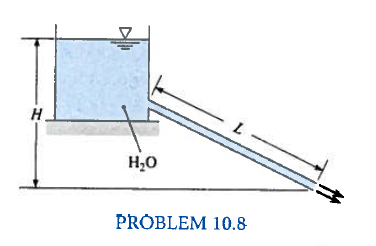
\includegraphics[width=3.5in]{TankDrainC.jpg} 
   \caption{Tank draining through a tube.}
   \label{fig:TankDrainC}
\end{figure}
\clearpage

\item (Problem 10-63 pg 400) Figure \ref{fig:PumpStorageB} is a schematic of a pumped-storage system.   If a flow of 0.10 $m^3/s$ of water is to be maintained in the system shown, what power must be added to the water by the pump?  The pipe is made of steel and is 15 $cm$ in diameter.
\begin{figure}[htbp] %  figure placement: here, top, bottom, or page
   \centering
   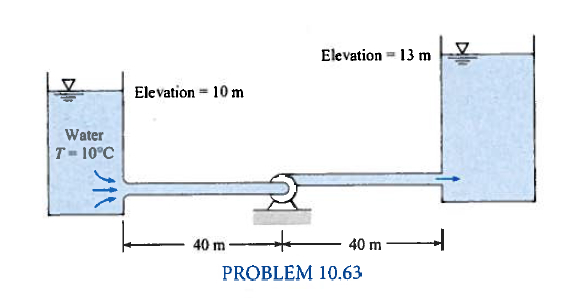
\includegraphics[width=4in]{PumpStorageB.jpg} 
   \caption{Pump-storage system}
   \label{fig:PumpStorageB}
\end{figure}
 

\end{enumerate}
\end{document}  